\chapter{Algorithms that Detect Interesting Higgs Boson Candidates}
\label{chap:four}
The analysis we perform will be looking for 2 Higgs bosons which decay into 4 total b quarks.
The 4b final state will decay into jets. 
Jets resulting from pairs of b quarks are identifiable because the parent Higgs jets are identifiable with a high degree of accuracy.
The following sections will detail how this is accomplished.
\section{Soft-Drop Mass Algorithm}

As previously stated, the decay signature of the Higgs boson we are looking for is a pair of b quarks.
When heavy particles, like the Higgs boson, decay to a pair of quarks, the angle between those two quarks is dependant only on the velocity of the parent heavy particle\footnote{This is for the lab frame. In the rest frame of the parent particle the two quarks will decay back to back.}.
Low energy Higgs will produced two distinct b quark jets where high energy Higgs will produce a collimated, also called ``boosted'', single jet.
Since we then are concerned with the energy of the parent particle, it is important for us to accurately determine if we are looking at the parent particle or not.
If you recall, pileup causes jets from background processes to appear to have the same mass\footnote{We will sometimes substitute mass and energy freely since the lorentz invariant mass is also useful to measure as a proxy for energy.} as a jet from a heavier particle.
Of the grooming algorithms that exist to differentiate these two cases, we will use the \textit{Soft-Drop Mass Algorithm}.

The algorithm starts by unclustering the jet, recall we cluster jet with the Anti-$k_T$ algorithm, and then categorizing the constituents as pseudo-jets.
These pesudo-jets are then compared to each other using the formula:
\begin{equation}
    \frac{min(p_{T,1},p_{T,2})}{p_{T,1}+p_{T,3}} > z
\end{equation}
where $z$ determines the strength of the cut. Our analysis uses $z = 0.1$\textbf{CHECK THIS} as the cut. 
If this condition is true, then the jet is kept. Otherwise, it is thrown out for consideration as a heavy particle jet.
This helps mimic the conditions that a real heavy particle would cause rather than those that come from pileup.
Since we use this as a discriminator for heavy particle jets and their decays, we will use it as a tagging variable in our analysis.

\section{Deep AK8 Mass Decorrelated Tagger}

Anotehr way to tag Higgs bosons is through exploiting the information that is gained when creating particle flow candidates and using a machine learning algorithm to identify hadronically decaying heavy particles, like the Higgs boson.
The algorithm also further delineates the decay product into decay modes, i.e. a Higgs to two b quarks. This algorithm is called \textit{Deep-AK8}.
The algorithm begins by defining two lists of inputs. The first list is a list of 100\footnote{Typically, jets do not have more than 100 constituent particles so using this cap contributes to a negligible loss of information.} jet constituent particles list in decreasing $p_T$.
Measured properties of each particle, $p_T$, the energy deposit, the charge, the angular separation between the particle and the
jet axis, etc., are used to help the algorithm extract features related to the substructure of the jet.
Charged particle will also have information from tracking including track quality and displacement.
These features are especially useful for identifying heavy flavour quarks, like the b quark. In total there are 42 pieces of information for each particle in the list.

The second list is comprised of secondary vertex information. Recall that the primary vertex relates to the location of the initial proton-proton collision.
The secondary vertex relates to the location of the next decay. So then this can be useful for identifying decaying products.
Notably, the b quark has a longer lifetime than other quarks, so its decay vertex, the secondary vertex, is very useful in its identification. This is shown pictorially in Figure \ref{fig:fig_4-1}.
This list will contain up to 7 secondary vertices as well as kinematic information about the vertices, displacement, and quality of the vertices.
Since this is a large amount of information, it poses a challenge to directly using it. The correlation between these inputs is very important for identifying particles so a custom neural network architecture is used.

\begin{figure} %  figure placement: here, top, bottom, or page
    \centering
 %   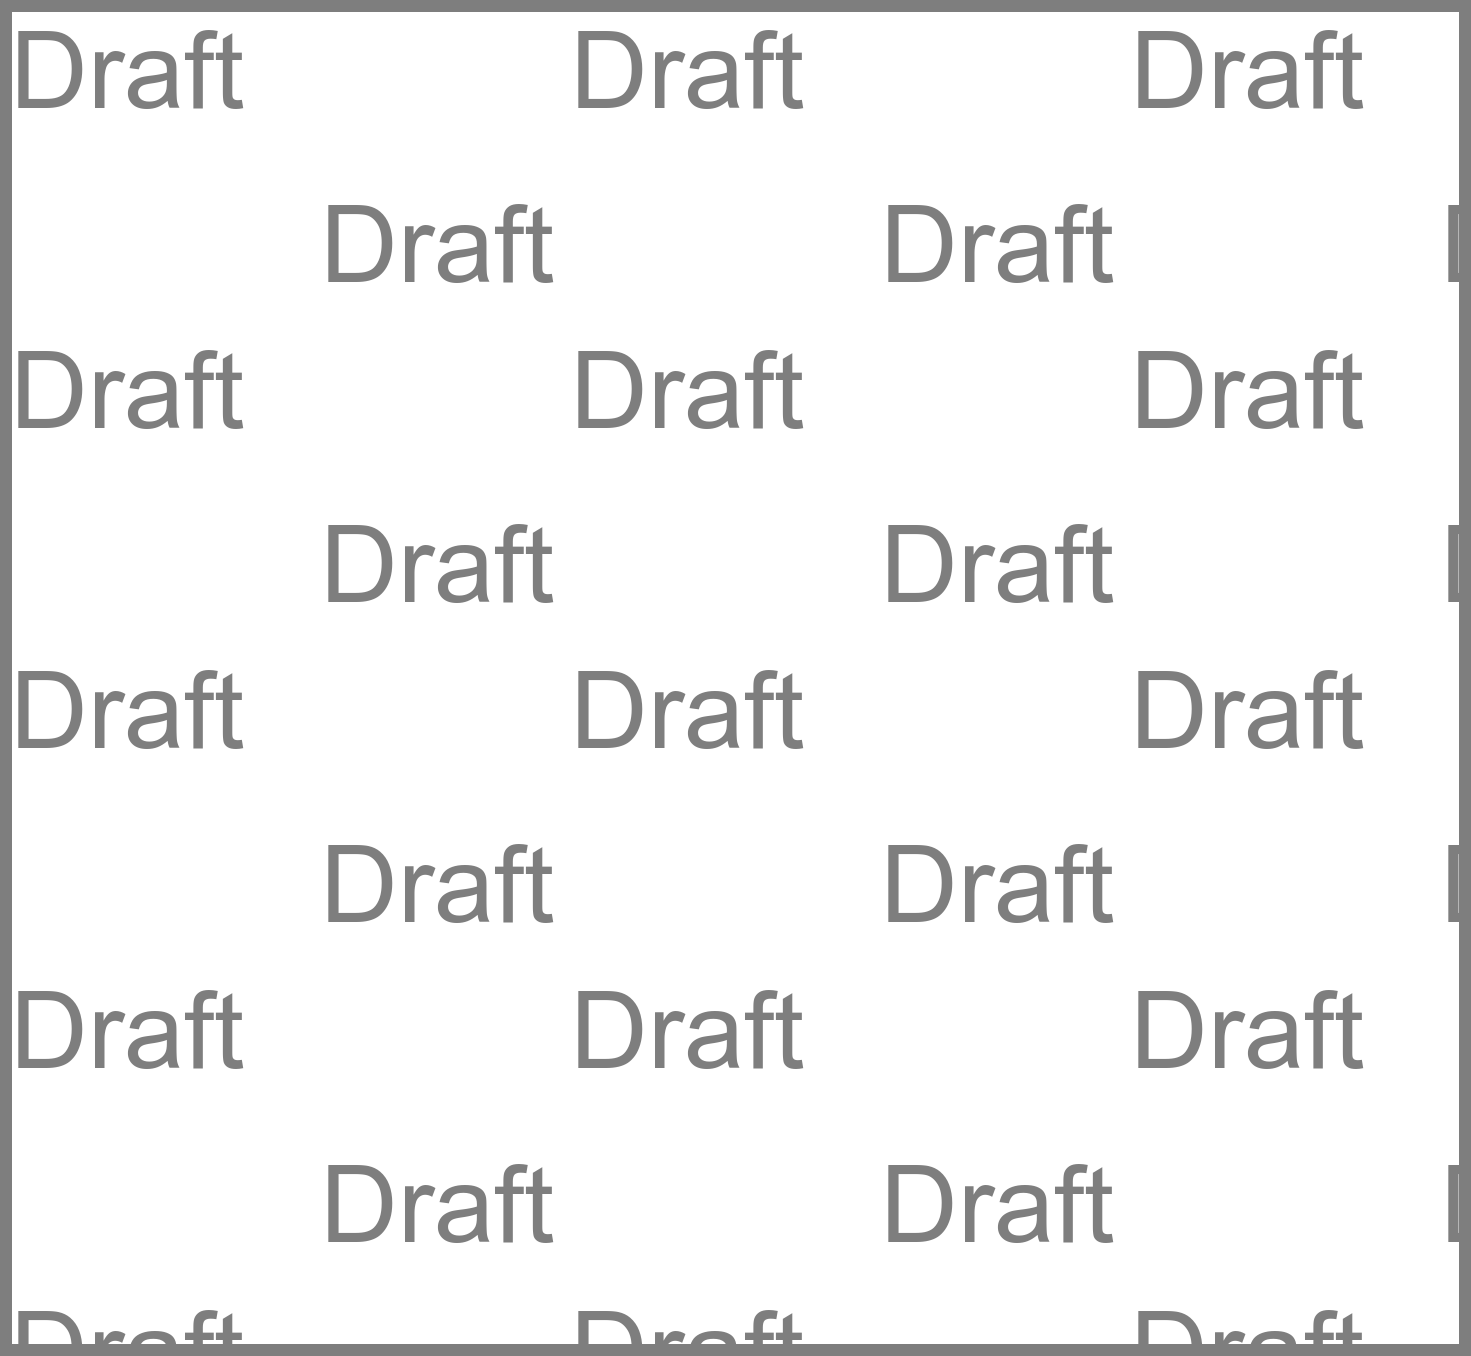
\includegraphics[width=\textwidth,height=\textheight,keepaspectratio]{fig_2-1}
    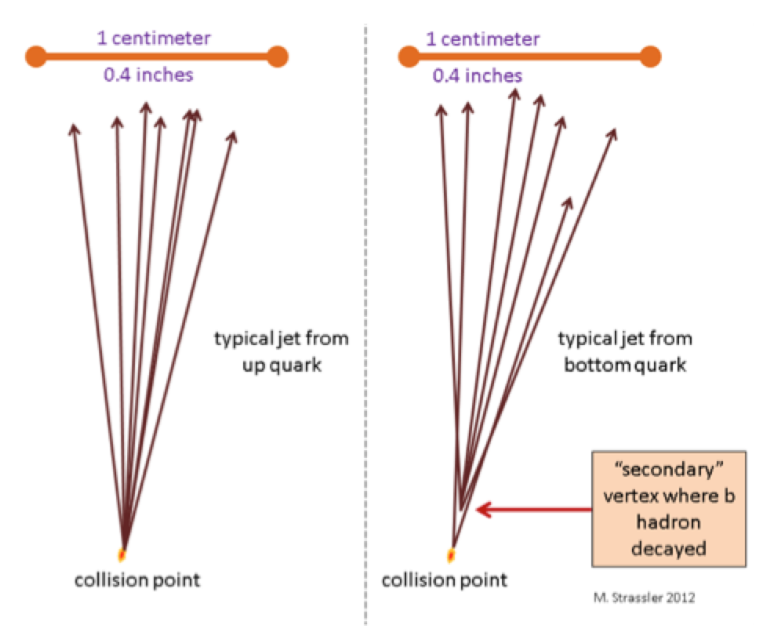
\includegraphics[scale=0.5]{bquarkSV.png}
    \caption{A diagram of how quarks behave in the detector.}
    \label{fig:fig_4-1}
 \end{figure}
\subsection{Custom Neural Network}

A custom deep neural network (DNN) is constructed in order to handle the complicated correlations between inputs.
This consists of two steps. The first step is to apply a convolutional neural network (CNN) is used to process each of the two lists in parallel.
Then in the second step, the output of the CNN is combined by a simple, fully connected network to perform the classification of the jet.
A re-weighting is used avoid any dependance on jet $p_T$ that can occur when training the network with a mix of background and signal samples.
The network architecture is shown in Figure \ref{fig:fig_4-2}.
\begin{figure} %  figure placement: here, top, bottom, or page
    \centering
 %   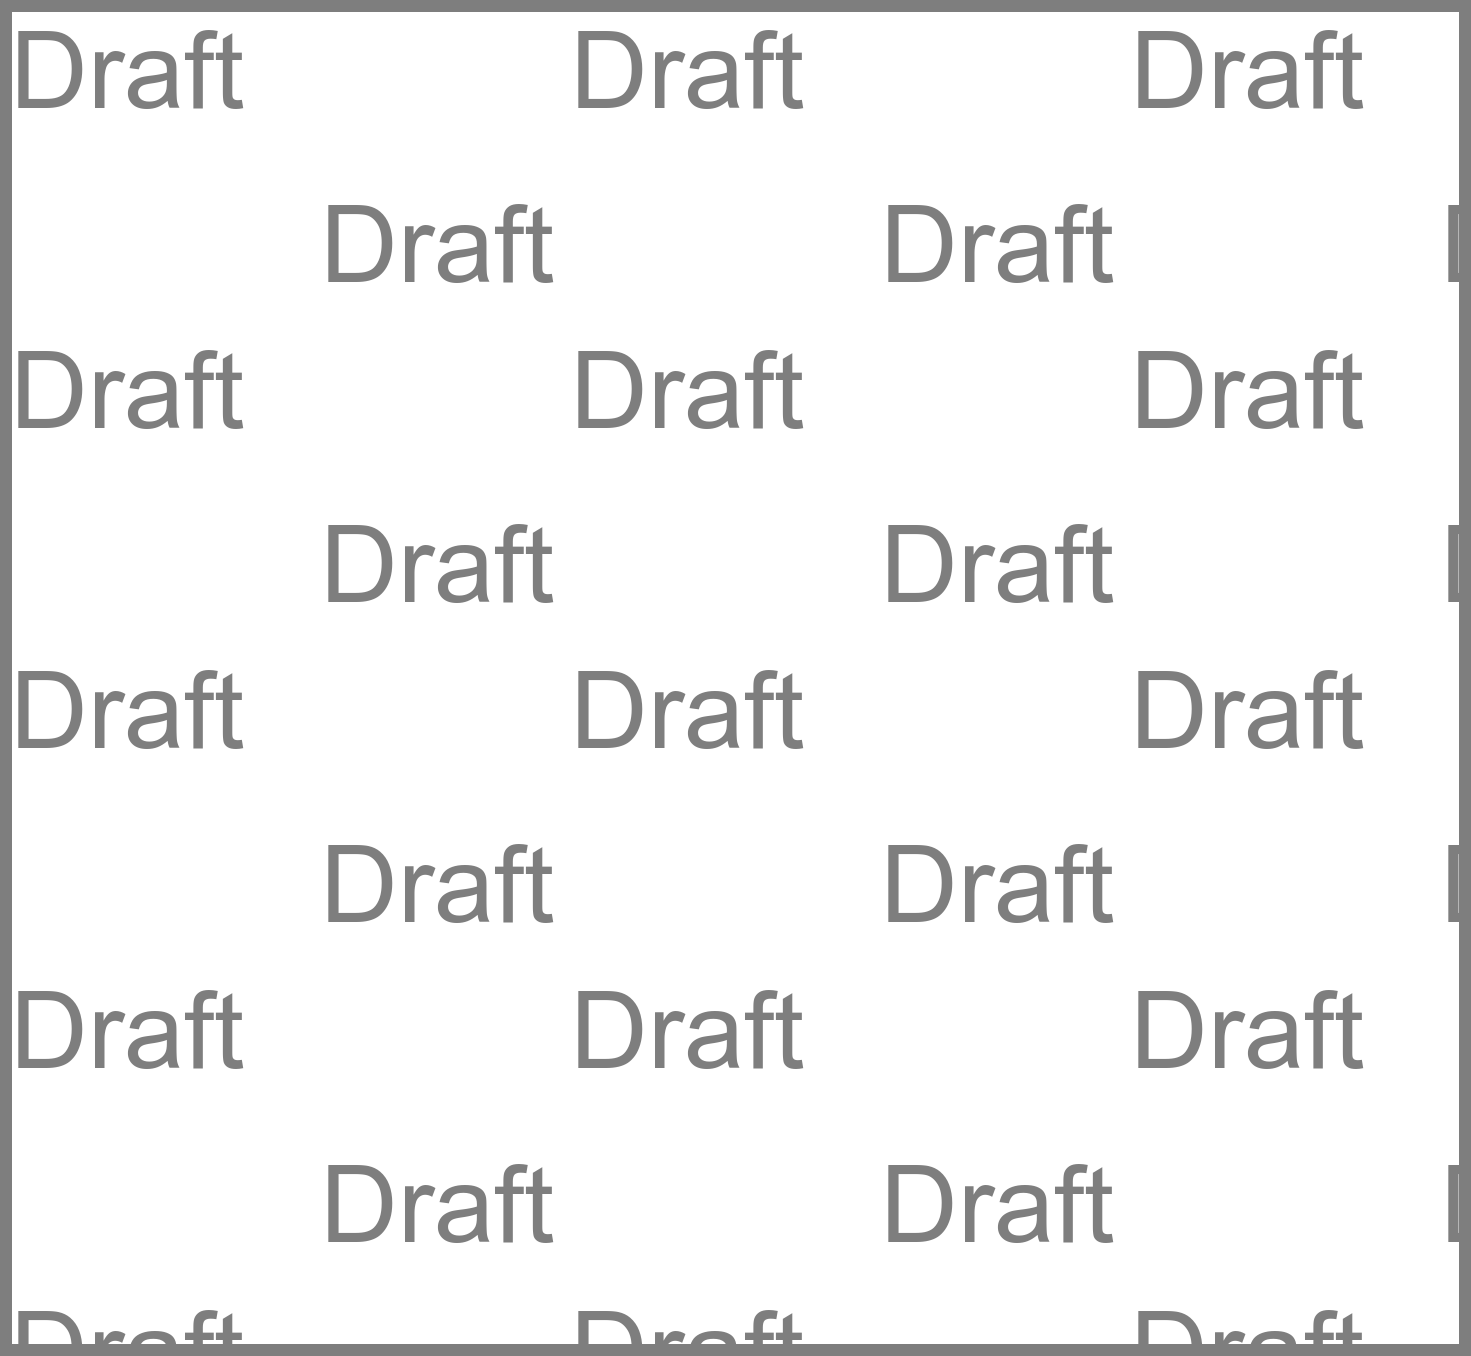
\includegraphics[width=\textwidth,height=\textheight,keepaspectratio]{fig_2-1}
    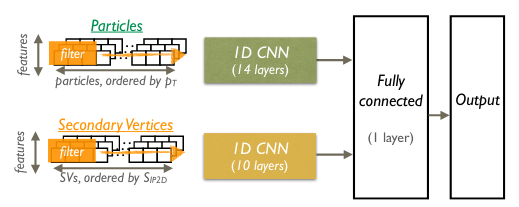
\includegraphics[scale=0.7]{deepAK8Arch.png}
    \caption{A diagram of the network architecture of the DeepAK8 Algorithm.}
    \label{fig:fig_4-2}
 \end{figure}
\subsection{Custom Neural Network}
If one wants to use mass as a discriminating variable, then a mass-decorrelated version of the DeepAK8 algorithm is used.
This will add a feature to the network architecture that acts as a mass prediction score. This score then acts as a penalty weight to prevent the network from extracting features that correlate with mass.
This allows the algorithm to become largely mass independent. This will decrease the power of the algorithm. The network architecture is shown in Figure \ref{fig:fig_4-3}.
The training of the DeepAK8-MD tagger was conducted on jets with a softdrop mass ($m_{SD})$ between 30 and 250 $GeV$ so any jet outside of that range should not be used in conjunction with this algorithm.
\begin{figure} %  figure placement: here, top, bottom, or page
    \centering
 %   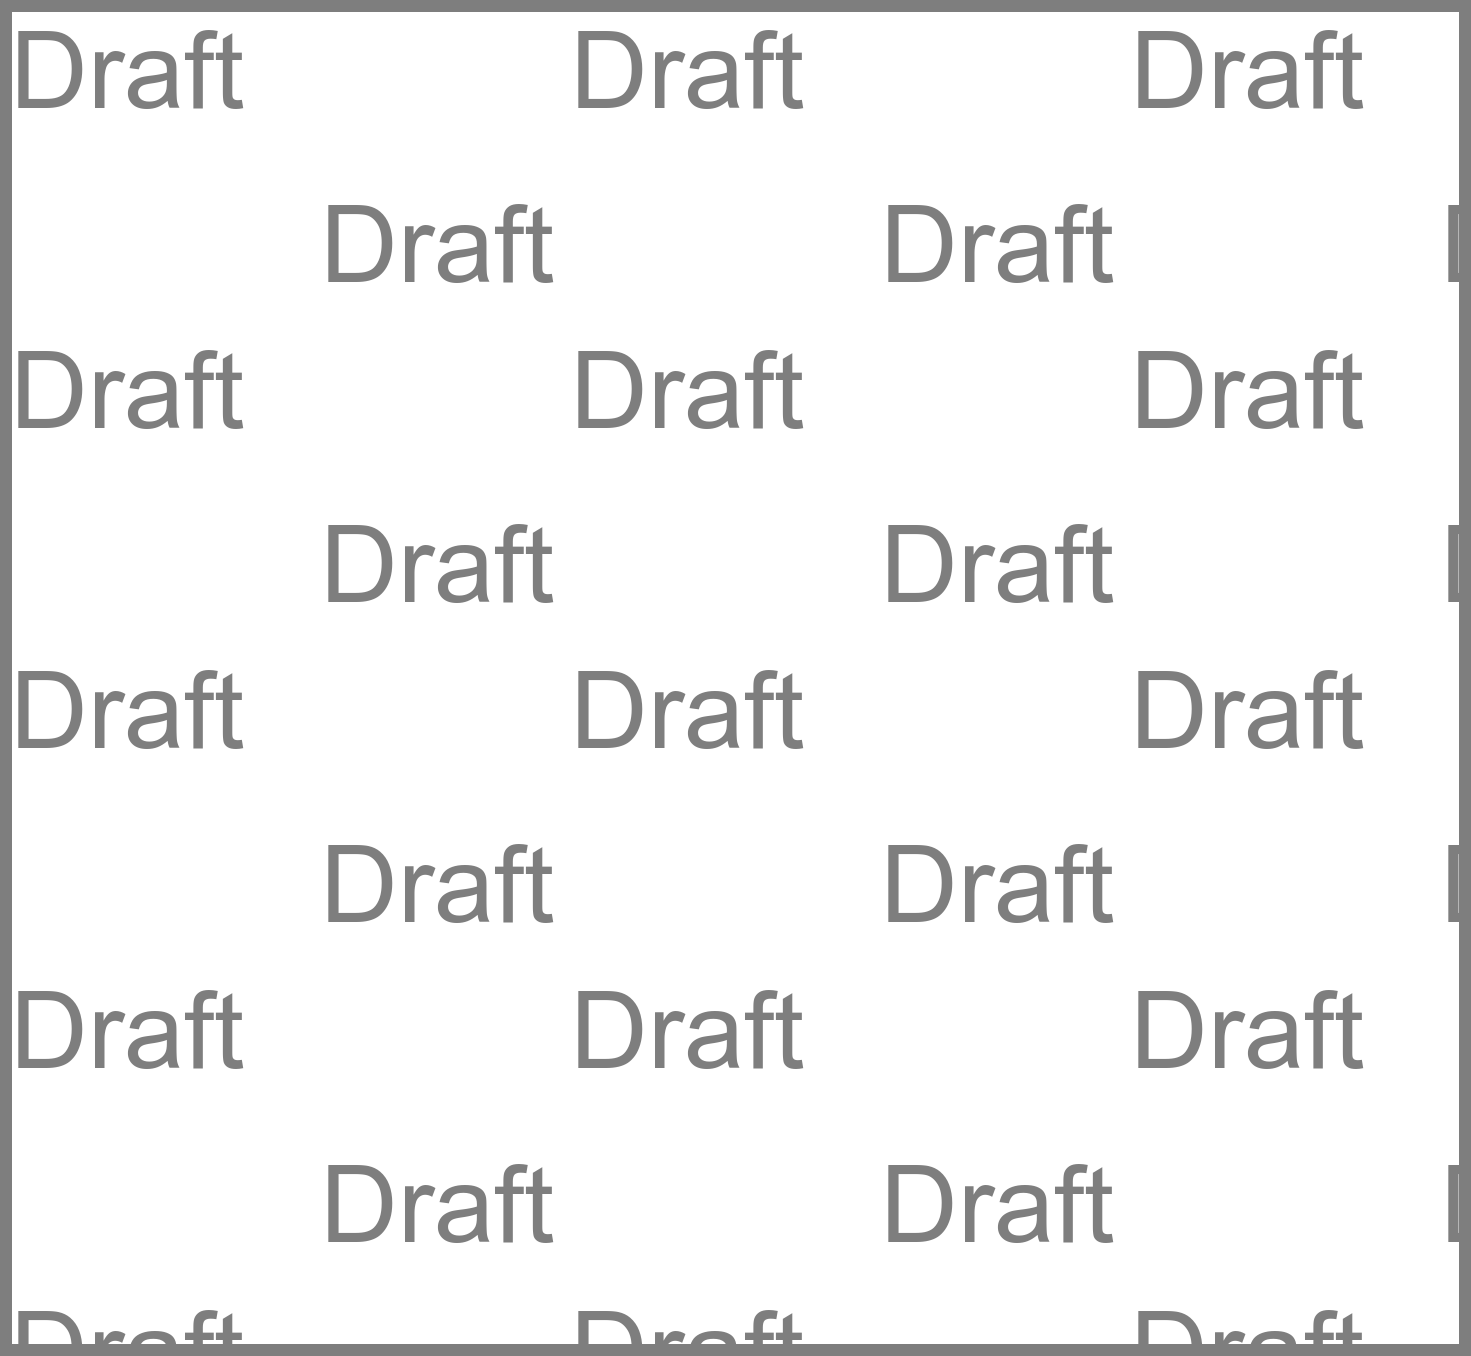
\includegraphics[width=\textwidth,height=\textheight,keepaspectratio]{fig_2-1}
    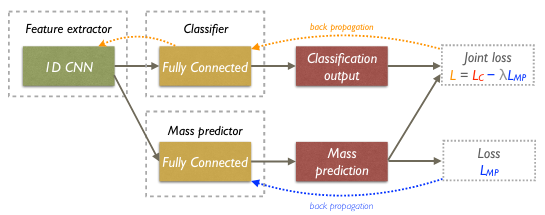
\includegraphics[scale=0.7]{deepAK8MDArch.png}
    \caption{A diagram of the network architecture for the Mass-Decorrelated version of the DeepAK8 Algorithm.}
    \label{fig:fig_4-3}
 \end{figure}

\subsection{Advantages}

A similar analysis to the one performed in this analysis was completed with a different tagging algorithm and on only the 2016 data.
This ``Double B'' tagger worked by using a boosted decision tree learning algorithm to assign a score to the jet measuring the likelihood that it contains two b quarks.
It is also mass and $p_T$ independent. At the time of that analysis, it was the best performing tagger available. However, it had drawbacks.
The biggest drawback is that, while it attempted to use jet substructure information, it needed to be supplemented with directly measured substructure variables.
The penalty is paid in the systematic uncertainty of those variables, which unfortunately is relatively high.
The DeepAK8 tagger uses those substructure variables more efficiently so we can actually drop them as an extra discriminator and avoid paying the same penalty.

\section{Deep Jet Tagger}

The Deep Jet algorithm is used to find jets that are not pairs of b quarks but individual b quarks, i.e AK4 jets. 
It uses a similar two network structure like the DeepAK8 algorithm but substitutes a recurrent neural network (RNN) instead of using the simple fully connected network that DeepAK8 uses.
It starts by training the CNN on separate collections of charged and neutral jet particle flow candidates. 
The outputs are then fed into the RNN. After that training, the resultant output is combined with variables such as $p_T$ and $\eta$ of each jet and then processed by a dense layer with 7 hidden layers.
The network architecture is shown in Figure \ref{fig:fig_4-4}
A score is then given based on the likelihood of the decay product being a heavy flavour quark. The improvement over the algorithm previously used to identify AK4 jets, called Deep CSV, is gained by using a larger set of inputs and a better neural network model.
\begin{figure} %  figure placement: here, top, bottom, or page
    \centering
 %   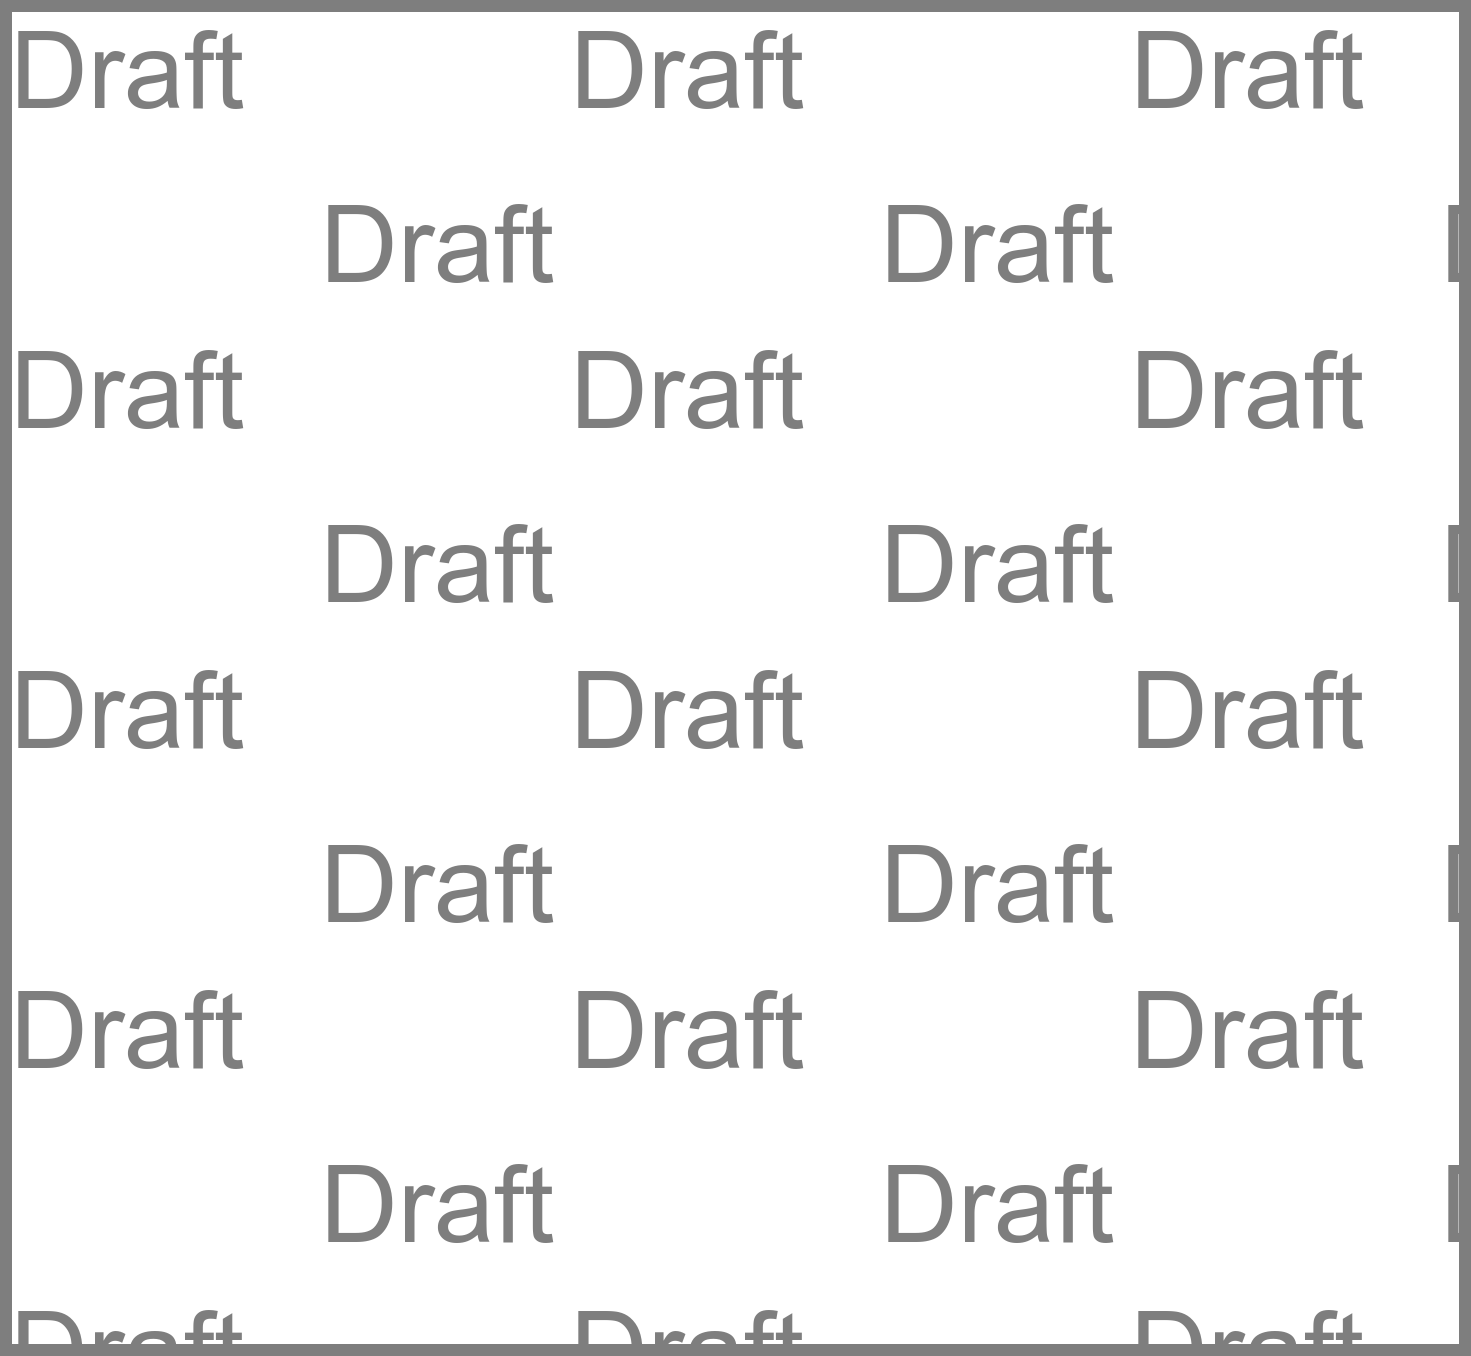
\includegraphics[width=\textwidth,height=\textheight,keepaspectratio]{fig_2-1}
    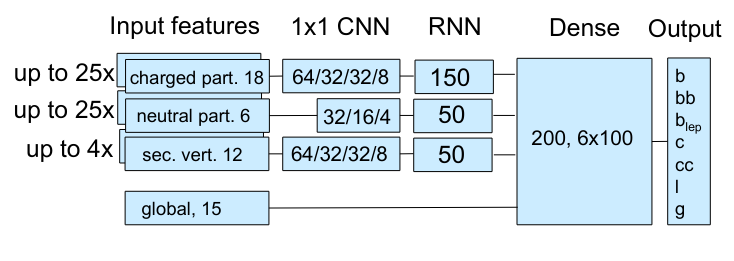
\includegraphics[scale=0.5]{deepJetArch.png}
    \caption{A diagram of the network architecture for the Deep Jet Algorithm.}
    \label{fig:fig_4-4}
 \end{figure}
